\section{Telemetry} \label{sec:telemetry}

All telemetry messages are designed to be sent over UDP using multicast functionality. This will allow the server
implementation to send a single UDP message which can be delivered to all subscribers.

In addition, the use of the UDP protocol is well-suited for telemetry applications. Measurements are made and
transmitted multiple times in a tenth of a second. It is not worth the overhead of TCP to have acknowledgements for each
of these messages, since if one is lost many will follow and the information will become obsolete quickly.

The multicast address for telemetry is \texttt{224.0.0.10}, using port \texttt{50002}.

\subsection{Measurements}

The hybrid control system measures three key pieces of information:

\begin{enumerate}
    \item Temperature
    \item Pressure
    \item Mass
\end{enumerate}

These measurements give the operator insight into whether or not the system is becoming unstable, if filling is
proceeding nominally, etc.

All measurements are only temporally valid, so they must be associated with a time stamp indicating the time of
measurement.

\subsubsection{Temperature} \label{sec:temperature}

\begin{figure}[H]
    \centering
    \begin{bytefield}{32}
        \bitheader{0-31} \\
        \wordbox{1}{Time} \\
        \wordbox{1}{Temperature} \\
        \bitbox{8}{ID} \\
    \end{bytefield}
    \caption{Temperature measurement format}
\end{figure}

\textbf{Time:} A time stamp measured in milliseconds since the system received power. This field is an unsigned 32-bit
integer.

\textbf{Temperature:} Temperature measured in millidegrees Celsius. This field is a signed 32-bit integer.

\textbf{ID:} The numerical ID of the sensor which took the measurement. This field is an unsigned 8-bit integer.

\subsection{Pressure} \label{sec:pressure}

\begin{figure}[H]
    \centering
    \begin{bytefield}{32}
        \bitheader{0-31} \\
        \wordbox{1}{Time} \\
        \wordbox{1}{Pressure} \\
        \bitbox{8}{ID} \\
    \end{bytefield}
    \caption{Pressure measurement format}
\end{figure}

\textbf{Time:} A time stamp measured in milliseconds since the system received power. This field is an unsigned 32-bit
integer.

\textbf{Pressure} Pressure measured in thousandths of PSI (milli-PSI). This field is an unsigned 32-bit integer.

\textbf{ID:} The numerical ID of the sensor which took the measurement. This field is an unsigned 8-bit integer.

\subsubsection{Mass} \label{sec:mass}

\begin{figure}[H]
    \centering
    \begin{bytefield}{32}
        \bitheader{0-31} \\
        \wordbox{1}{Time} \\
        \wordbox{1}{Mass} \\
        \bitbox{8}{ID} \\
    \end{bytefield}
    \caption{Mass measurement format}
\end{figure}

\textbf{Time:} A time stamp measured in milliseconds since the system received power. This field is an unsigned 32-bit
integer.

\textbf{Mass} Mass measured in grams. This field is an unsigned 32-bit integer.

\textbf{ID:} The numerical ID of the sensor which took the measurement. This field is an unsigned 8-bit integer.

\subsection{Arming State} \label{sec:arming-state}

The hybrid control system's arming state should be known at all times over telemetry.

\begin{figure}[H]
    \centering
    \begin{bytefield}{32}
        \bitheader{0-31} \\
        \wordbox{1}{Time} \\
        \bitbox{8}{State} \\
    \end{bytefield}
    \caption{Arming state message format}
\end{figure}

\textbf{Time:} A time stamp measured in milliseconds since the system received power. This field is an unsigned 32-bit
integer.

\textbf{State:} The arming state of the control system.

\begin{table}[H]
    \centering
    \begin{tabular}{| c | c | p{3.5in} |}
        \hline
        State               & Value & Description                                                                              \\
        \hline
        ARMED\_PAD          & 0     & The pad control box is armed.                                                            \\
        \hline
        ARMED\_VALVES       & 1     & The control input box is armed, permitting control over solenoid valves.                 \\
        \hline
        ARMED\_IGNITION     & 2     & The pad control box is armed, connecting power to ignition circuity. Actuating the quick
        disconnect is now permitted.                                                                                           \\
        \hline
        ARMED\_DISCONNECTED & 3     & The quick disconnect is disconnected. Commands to ignite the ignitor are now permitted.  \\
        \hline
        ARMED\_LAUNCH       & 4     & The ignitor is lit. Commands to open the fire valve are now permitted.                   \\
        \hline
    \end{tabular}
    \caption{Valid arming states}
    \label{tbl:arming-states}
\end{table}



\subsection{Actuator State} \label{sec:act-state}

The state of the hybrid control system's actuators should be known at all times over telemetry.

\begin{figure}[H]
    \centering
    \begin{bytefield}{32}
        \bitheader{0-31} \\
        \wordbox{1}{Time} \\
        \bitbox{8}{ID}
        \bitbox{8}{State} \\
    \end{bytefield}
    \caption{Actuator state message format}
\end{figure}

\textbf{Time:} A time stamp measured in milliseconds since the system received power. This field is an unsigned 32-bit
integer.

\textbf{ID:} The unique numerical ID of the actuator whose state is being sent in this message.

\textbf{State:} The state of the actuator. See Table \ref{tbl:actuator-states} for the valid actuator states.

\begin{table}[H]
    \centering
    \begin{tabular}{| c | c | c |}
        \hline
        State & Value & Description                    \\
        \hline
        OFF   & 0     & The actuator is off, or close. \\
        \hline
        ON    & 1     & The actuator is on, or open.   \\
        \hline
    \end{tabular}
    \caption{Valid actuator states}
    \label{tbl:actuator-states}
\end{table}

\begin{table}
    \centering
    \begin{tabular}{| c | c | p{3in} |}
        \hline
        Actuator Name    & ID & Description                                                              \\
        \hline
        Fire Valve       & 0  & Servo motor on valve which release oxidizer onto flame.                  \\
        \hline
        XV-1             & 1  & Solenoid valve                                                           \\
        \hline
        XV-2             & 2  & Solenoid valve                                                           \\
        \hline
        XV-3             & 3  & Solenoid valve                                                           \\
        \hline
        XV-4             & 4  & Solenoid valve                                                           \\
        \hline
        XV-5             & 5  & Solenoid valve                                                           \\
        \hline
        XV-6             & 6  & Solenoid valve                                                           \\
        \hline
        XV-7             & 7  & Solenoid valve                                                           \\
        \hline
        XV-8             & 8  & Solenoid valve                                                           \\
        \hline
        XV-9             & 9  & Solenoid valve                                                           \\
        \hline
        XV-10            & 10 & Solenoid valve                                                           \\
        \hline
        XV-11            & 11 & Solenoid valve                                                           \\
        \hline
        XV-12            & 12 & Solenoid valve                                                           \\
        \hline
        Quick disconnect & 13 & The quick disconnect to separate ground system plumbing from the rocket. \\
        \hline
        Igniter          & 14 & The igniter that starts the flame for launch                             \\
        \hline
    \end{tabular}
    \caption{Agreed actuator IDs}
    \label{tbl:act-ids}
\end{table}

\subsection{Warnings} \label{sec:warnings}

Warnings are issued when measurements exceed a certain threshold.

\begin{figure}[H]
    \centering
    \begin{bytefield}{32}
        \bitheader{0-31} \\
        \wordbox{1}{Time} \\
        \bitbox{8}{Type} \\
    \end{bytefield}
    \caption{Warning message format}
\end{figure}

\textbf{Time:} A time stamp measured in milliseconds since the system received power. This field is an unsigned 32-bit
integer.

\textbf{Type:} The warning type. A list of valid types can be found in Table \ref{tbl:warnings}.

\begin{table}[H]
    \centering
    \begin{tabular}{| c | c | p{3.5in} |}
        \hline
        \textbf{Name}  & \textbf{Value} & \textbf{Description}                                                                        \\
        \hline
        HIGH\_PRESSURE & 0              & Pressure levels have exceeded the warning threshold and manual intervention is required.    \\
        \hline
        HIGH\_TEMP     & 1              & Temperature levels have exceeded the warning threshold and manual intervention is required. \\
        \hline
    \end{tabular}
    \caption{Warning types}
    \label{tbl:warnings}
\end{table}



\section{Arming Logic}
The control logic that the pad server uses to govern which actuation and arming commands are valid at any given time are based on the arming state in Figure 13.

\begin{figure}[H]
	\centering
	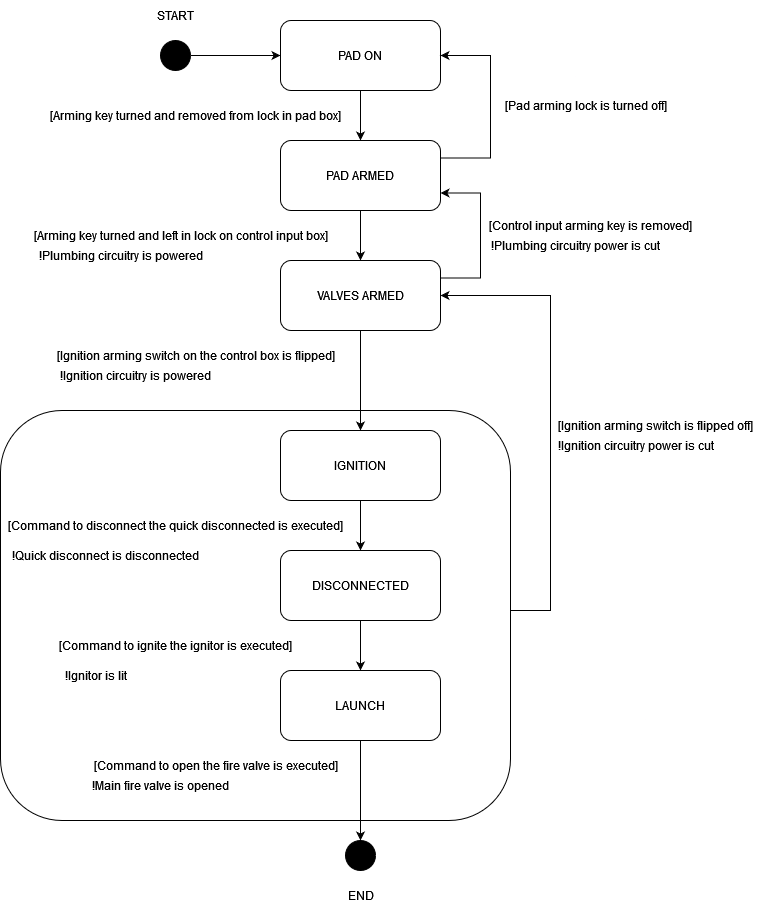
\includegraphics[width=4in]{./assets/Hybrid_Control_FSM.png}
	\caption{Logging control}
	\label{fig:logging-fsm}
\end{figure}


\begin{table}[H]
	\centering
	\begin{tabular}{| c | c |}
		\hline
		State               & Available Actuators                                                                             \\
		\hline
		ARMED\_PAD                    & None                                             \\
		\hline
		ARMED\_VALVES                & XV-1...XV12        \\
		\hline
		ARMED\_IGNITION          & Quick Disconnect, XV-1...XV12                                                                                    \\
		\hline
		ARMED\_DISCONNECTED  & Igniter, XV-1...XV12                   \\
		\hline
		ARMED\_LAUNCH               & Fire Valve, XV-1...XV12          \\
		\hline
	\end{tabular}
	\caption{Available Actuators for each arming state}
	\label{tbl:available-actuators}
\end{table}
